\begin{figure}[H]\centering
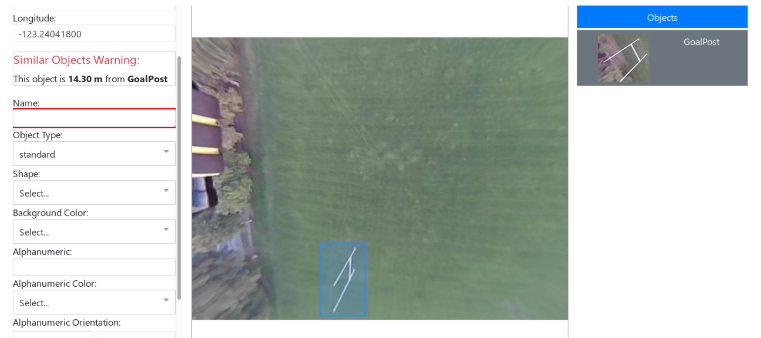
\includegraphics[width=\linewidth]{figures/ODLC1}
\caption{Object Detection and Classification Interface}
\label{fig:ODLC1}
\end{figure}

The ODLC (Object Detection, Localization, Classification) task is handled by GCOMv2’s IMP (Image Processing) module. The IMP module consists of a frontend web UI (User Interface) and a corresponding backend module in GCOMv2’s web server. Whenever a new image is transferred to the server computer, IMP extracts the relevant image and aircraft data (latitude, longitude, altitude, heading, and aircraft roll) and preprocesses the image. See figure \ref{fig:ODLC1}.

\begin{figure}[H]\centering
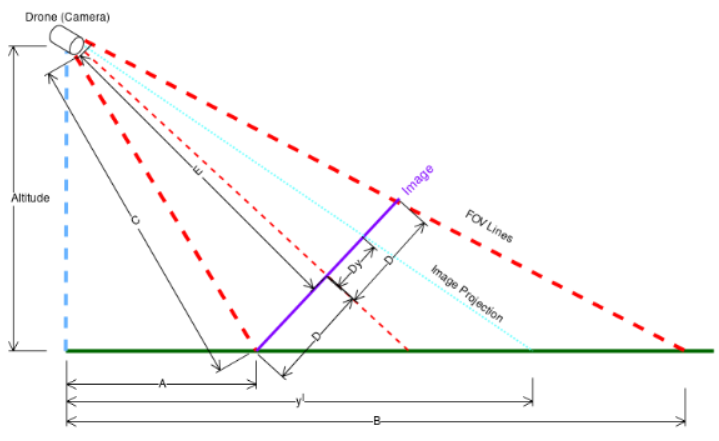
\includegraphics[width=\linewidth]{figures/ODLC2}
\caption{Object Localization Algorithm Diagram}
\label{fig:ODLC2}
\end{figure}

\onecolumn

\begin{figure*}[h]\centering
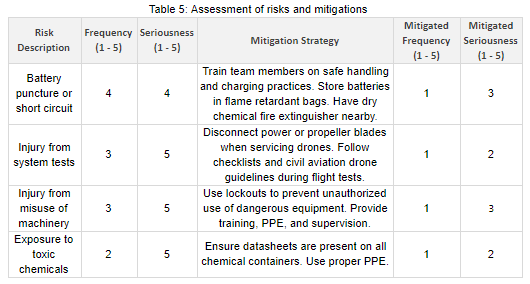
\includegraphics[width=0.75\linewidth]{table/Table_5_Assessment_of_risks_and_mitigations.PNG}
\caption*{}
\label{fig:Table_5_Assessment_of_risks_and_mitigations}
\end{figure*}

\begin{figure*}[h]\centering
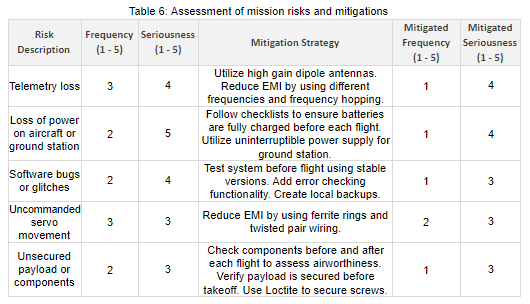
\includegraphics[width=0.75\linewidth]{table/Table_6_Assessment_of_mission_risks_and_mitigations.PNG}
\caption*{}
\label{fig:Table_6_Assessment_of_mission_risks_and_mitigations}
\end{figure*}

\twocolumn

To adjust for the roll of the aircraft, in the absence of a gimbal for that axis, trigonometry is used to ensure that the location of the ODLC is as accurate as possible. The image is mapped in 3D space based on the roll, altitude and FOV of the camera. The object location inside the image is then projected from the camera, through the mapped image and onto the ground plane to determine the exact location in real space. This process is done in both the x and y dimensions. Due to the gimbal, the correction really only applies to the image y direction, however because the image is larger than a single point, the x dimension gets a small correction even with an angle of 0.  The calculations for figure \ref{fig:ODLC2} are in the following order, let $\Omega$  = image's relative altitude, $I_h$ = image's height in pixel and $\theta_x$ = x's facing angle:
\begin{align*}
C & = \sqrt{\Omega^2+(\Omega \cdot tan(\theta_A))^2}
\\D & =|C \cdot sin(\theta_D)| \\
y & = y_{px} \cdot \frac{2D}{ I_h}  \label{eq:odlc_eq_1}\tag{1}
\\ \theta_y & = atan(\frac{y-D}{\sqrt{C^2-D^2}})
\\y'& = \Omega \cdot tan(\theta _y) \label{eq:odlc_eq_2}\tag{2}
\end{align*}
\eqref{eq:odlc_eq_1} $y$ represents the height of the target pixel in meters. This is originally in pixels from the bottom of the image, but is converted to meters in space. \\
\eqref{eq:odlc_eq_2} $y'$ is the horizontal offset of the objects real location from the drone location. Based off the heading of the drone this offset is added and the gps position adjusted accordingly.

In order to ensure that all images can be processed in the allotted time, the IMP UI allows for simultaneous processing on multiple computers. Each user is able to analyze a subset of the images in which they can draw a bounding box around any object, which computes the center and size of the object relative to the image. This data is sent to the server, where the GPS adjustment is applied to calculate the real GPS location and crop the image. The UI is especially designed for AUVSI SUAS, and allows users to easily classify the required characteristics of each object. See Figure 10 for an overall image processing system diagram.

To ensure that every object is detected once and only once, the IMP UI displays a list of all existing objects along with their cropped thumbnails. In addition, any user that tags an object within a range of any other object is notified for possible similarities. Each user is also able to flag any image that they deem unclear for other users to analyze.

\begin{figure}[H]\centering
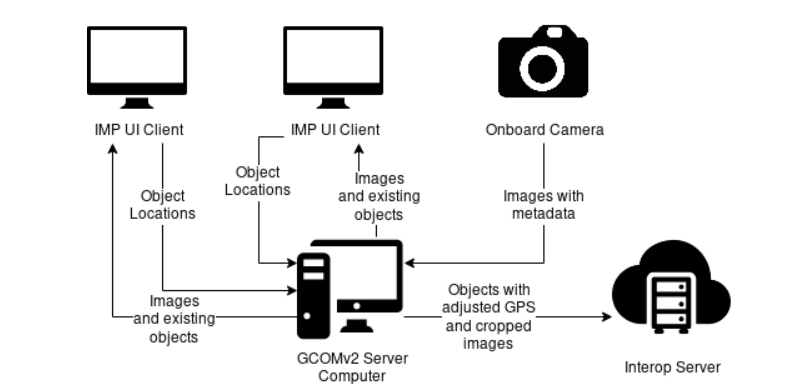
\includegraphics[width=\linewidth]{figures/ODLC3}
\caption{Image Processing System Diagram }
\label{fig:ODLC3}
\end{figure}

Every aspect of the ODLC pipeline was heavily unit-tested to ensure that all calculations were correct for different inputs, such as variability in image sizes, object locations, and aircraft speed and positions. Then the system was tested as a whole, by placing test objects at known GPS locations, and verifying that images were taken, transferred, identified, and correctly sent to Interop.



\endinput